\begin{examplebox}
\textbf{例1：直接计算（保留原例）}
已知 $R=3,OP=5$，求圆周距离最值。\begin{center}
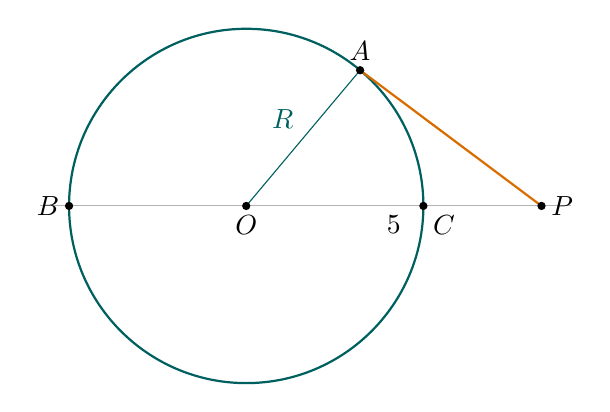
\begin{tikzpicture}[scale=.75,>=stealth]
 \coordinate (O) at (0,0); \coordinate (P) at (5,0);
 \coordinate (A) at (50:3); \coordinate (C) at (3,0); \coordinate (B) at (-3,0);
 \draw[gray!60] (-3.5,0)--(5.5,0);
 \draw[teal!75!black,thick] (O) circle (3);
 \draw[teal!75!black] (O)--(A) node[midway,above left] {$R$};
 \draw[orange!85!black,thick] (P)--(A);
 \fill (O) circle (2pt) node[below] {$O$};
 \fill (P) circle (2pt) node[right] {$P$};
 \fill (A) circle (2pt) node[above] {$A$}; \path (O)--(P) node[midway,below] {$5$}; \fill (C) circle (2pt) node[below right] {$C$}; \fill (B) circle (2pt) node[left] {$B$};
 \end{tikzpicture}

\end{center}
解：$5>3$，点在圆外。最小值 $5-3=2$，最大值 $5+3=8$。

\textbf{例2：坐标形式} 圆 $(x-1)^2+(y+2)^2=4$，定点 $P=(4,2)$，求距离最值及对应点。

圆心 $O=(1,-2)$，半径 $R=2$，$d=\sqrt{3^2+4^2}=5>2$。故最小值 $3$，最大值 $7$。

从 $O$ 指向 $P$ 的单位向量为 $(3/5,4/5)$，最近点 $C=(1,-2)+2(3/5,4/5)=(11/5,-2/5)$，最远点 $B=(1,-2)-2(3/5,4/5)=(-1/5,-18/5)$。\begin{center}
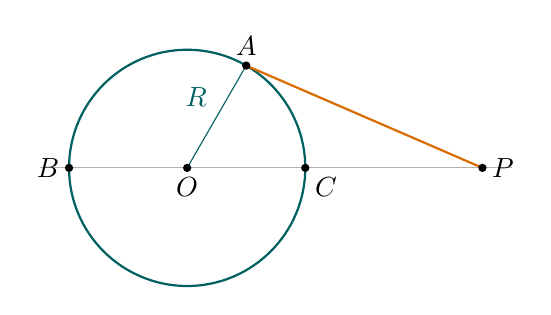
\begin{tikzpicture}[scale=.75,>=stealth]
 \coordinate (O) at (0,0); \coordinate (P) at (5,0);
 \coordinate (A) at (60:2); \coordinate (C) at (2,0); \coordinate (B) at (-2,0);
 \draw[gray!60] (-2.5,0)--(5.5,0);
 \draw[teal!75!black,thick] (O) circle (2);
 \draw[teal!75!black] (O)--(A) node[midway,above left] {$R$};
 \draw[orange!85!black,thick] (P)--(A);
 \fill (O) circle (2pt) node[below] {$O$};
 \fill (P) circle (2pt) node[right] {$P$};
 \fill (A) circle (2pt) node[above] {$A$}; \fill (C) circle (2pt) node[below right] {$C$}; \fill (B) circle (2pt) node[left] {$B$};
 \end{tikzpicture}

\end{center}

\textbf{例3：根式最值} 求 $f(t)=\sqrt{(3\cos t-5)^2+9\sin^2t}$ 的值域，$t\in\mathbb R$。

识别为圆 $x^2+y^2=9$ 上动点 $(3\cos t,3\sin t)$ 到 $(5,0)$ 的距离。$d=5,R=3$，故值域为 $[2,8]$。端点分别在 $t=2k\pi$ 与 $t=(2k+1)\pi$ 取得；连续性保证中间值均能取得。\begin{center}
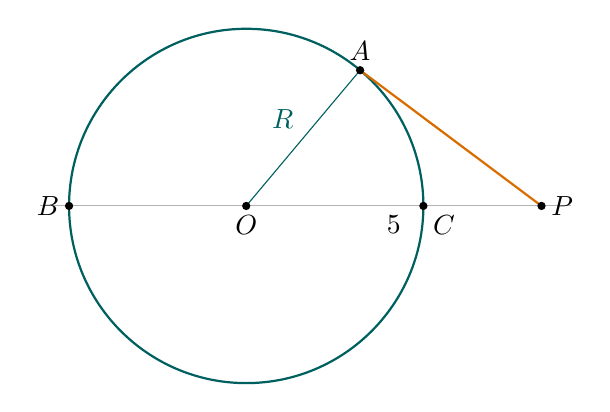
\begin{tikzpicture}[scale=.75,>=stealth]
 \coordinate (O) at (0,0); \coordinate (P) at (5,0);
 \coordinate (A) at (50:3); \coordinate (C) at (3,0); \coordinate (B) at (-3,0);
 \draw[gray!60] (-3.5,0)--(5.5,0);
 \draw[teal!75!black,thick] (O) circle (3);
 \draw[teal!75!black] (O)--(A) node[midway,above left] {$R$};
 \draw[orange!85!black,thick] (P)--(A);
 \fill (O) circle (2pt) node[below] {$O$};
 \fill (P) circle (2pt) node[right] {$P$};
 \fill (A) circle (2pt) node[above] {$A$}; \path (O)--(P) node[midway,below] {$5$}; \fill (C) circle (2pt) node[below right] {$C$}; \fill (B) circle (2pt) node[left] {$B$};
 \end{tikzpicture}

\end{center}

\textbf{变式训练} 圆 $x^2+y^2=4$ 上动点到 $(1,0)$ 的距离最值是多少？答案：$1,3$（点在圆内，不能直接使用外点最小值公式）。
\end{examplebox}
